%%%%%%%%%%%%%%%%%%%%%%%%%%%%%%%%%%%%%%%%%
% Dreuw & Deselaer's Poster
% LaTeX Template
% Version 1.0 (11/04/13)
%
% Created by:
% Philippe Dreuw and Thomas Deselaers
% http://www-i6.informatik.rwth-aachen.de/~dreuw/latexbeamerposter.php
%
% This template has been downloaded from:
% http://www.LaTeXTemplates.com
%
% License:
% CC BY-NC-SA 3.0 (http://creativecommons.org/licenses/by-nc-sa/3.0/)
%
%%%%%%%%%%%%%%%%%%%%%%%%%%%%%%%%%%%%%%%%%

%----------------------------------------------------------------------------------------
%	PACKAGES AND OTHER DOCUMENT CONFIGURATIONS
%----------------------------------------------------------------------------------------

\documentclass[final,hyperref={pdfpagelabels=false}]{beamer}

\usepackage[orientation=portrait,size=custom,width=100,height=150,,scale=1.8]{beamerposter} % Use the beamerposter package for laying out the poster with a portrait orientation and an a0 paper size

\usetheme{I6pd2} % Use the I6pd2 theme supplied with this template

\usepackage[english]{babel} % English language/hyphenation

\usepackage{amsmath,amsthm,amssymb,latexsym} % For including math equations, theorems, symbols, etc

%\usepackage{times}\usefonttheme{professionalfonts}  % Uncomment to use Times as the main font
%\usefonttheme[onlymath]{serif} % Uncomment to use a Serif font within math environments

\boldmath % Use bold for everything within the math environment

\usepackage{booktabs} % Top and bottom rules for tables

\graphicspath{{figures/}} % Location of the graphics files

\usecaptiontemplate{\small\structure{\insertcaptionname~\insertcaptionnumber: }\insertcaption} % A fix for figure numbering

\usepackage{natbib}

%----------------------------------------------------------------------------------------
%	TITLE SECTION 
%----------------------------------------------------------------------------------------

\title{\huge Testing Pleiotropy vs. Separate QTL in Multiparental Populations} % Poster title

\author{Frederick J. Boehm, Brian S. Yandell, and Karl W. Broman} % Author(s)

\institute{\small Departments of Statistics and of Biostatistics \& Medical Informatics, University of Wisconsin-Madison} % Institution(s)

%----------------------------------------------------------------------------------------
%	FOOTER TEXT
%----------------------------------------------------------------------------------------

\newcommand{\leftfoot}{} % Left footer text

\newcommand{\rightfoot}{} % Right footer text

%----------------------------------------------------------------------------------------

\begin{document}

\addtobeamertemplate{block end}{}{\vspace*{2ex}} % White space under blocks

\begin{frame}[t] % The whole poster is enclosed in one beamer frame

\begin{columns}[t] % The whole poster consists of two major columns, each of which can be subdivided further with another \begin{columns} block - the [t] argument aligns each column's content to the top

\begin{column}{.02\textwidth}\end{column} % Empty spacer column

\begin{column}{.465\textwidth} % The first column

%----------------------------------------------------------------------------------------
%	OBJECTIVES
%----------------------------------------------------------------------------------------

\begin{block}{Objectives}

\begin{enumerate}
\item Develop a test of pleiotropy vs. separate QTL in multiparental populations
\item Apply the test to behavioral traits in Diversity Outbred mice
\item Share software as an R package, \texttt{qtl2pleio}
\end{enumerate}

\end{block}

\begin{block}{A mouse on microarray chips}

\begin{figure}
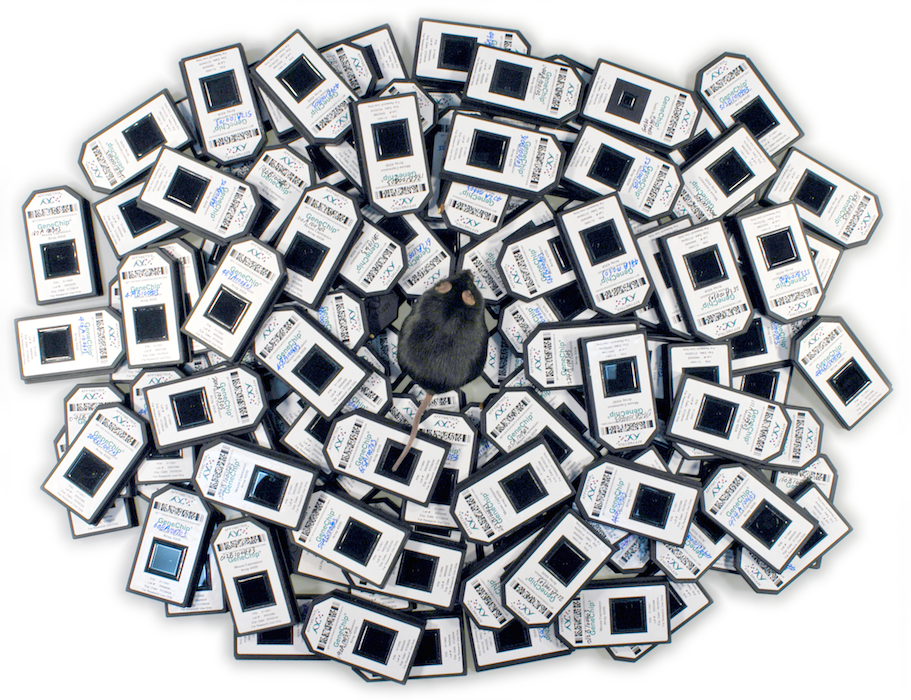
\includegraphics[width=0.42\linewidth]{mouse_on_chips.png}
\caption{\href{https://bit.ly/2DlQxPN}{https://bit.ly/2DlQxPN}
}
\end{figure}

\end{block}




%----------------------------------------------------------------------------------------
%	INTRODUCTION
%----------------------------------------------------------------------------------------
            
\begin{block}{Introduction}

\begin{itemize}
\item Multiparental populations enable high-resolution QTL mapping of biomolecular and clinical traits to inform systems genetics   
\item To better understand complex traits, new analysis tools, such as a test of pleiotropy vs. separate QTL, are needed 
\end{itemize}

\end{block}

%----------------------------------------------------------------------------------------
%	MATERIALS
%----------------------------------------------------------------------------------------


%----------------------------------------------------------------------------------------
%	METHODS
%----------------------------------------------------------------------------------------


%----------------------------------------------------------------------------------------
\begin{block}{Light-dark box}

\begin{figure}
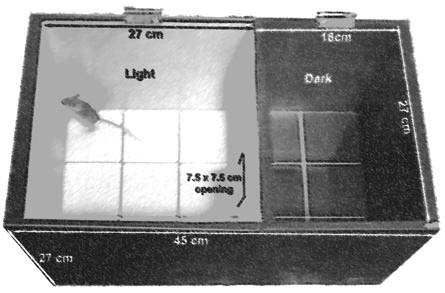
\includegraphics[width=0.5\linewidth]{lightdarkbox.jpg}
\caption{\href{https://phenome.jax.org/projects/Brown1/Protocol}{https://phenome.jax.org/projects/Brown1/Protocol}
}
\end{figure}

\end{block}
%----------------------------------------------------------------------------------------
\begin{block}{Behavioral genetics}
\begin{itemize}
\item \cite{logan2013high} and \cite{recla2014precise} examined 261 Diversity Outbred mice    
\item Identified \textit{Hydin} as the Chr 8 gene affecting "hot plate latency" at 57 cM    
\item Identified Chr 8 QTL for "percent time in light" and "distance traveled in light" at 55 cM    
\item Does \textit{Hydin} affect "percent time in light" and "distance traveled in light"?    
\end{itemize}

\end{block}




\begin{block}{Founder allele effects plots}
\begin{figure}
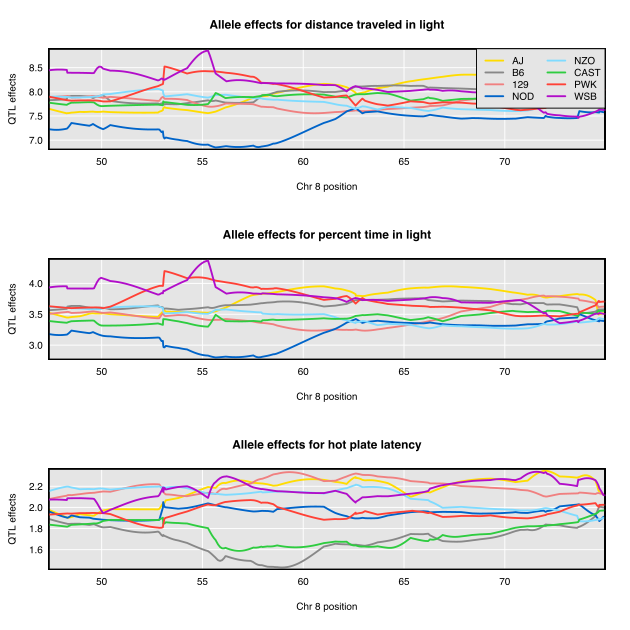
\includegraphics[width=0.5\linewidth]{coef_all3.png}
\caption{Founder allele effects for three traits \citep{macdonald2007joint}}
\end{figure}

\end{block}



%----------------------------------------------------------------------------------------

\end{column} % End of the first column

\begin{column}{.03\textwidth}\end{column} % Empty spacer column
 
\begin{column}{.465\textwidth} % The second column

%----------------------------------------------------------------------------------------
%	RESULTS
%----------------------------------------------------------------------------------------


\begin{block}{\cite{jiang1995multiple} test}
\begin{itemize}
  \item \cite{jiang1995multiple} developed a pleiotropy vs. separate QTL test for two-parent crosses
  \begin{itemize}
    \item $H_0$: pleiotropy vs. $H_A$: two separate QTL
    \item Perform a two-dimensional QTL scan   
    \item Calculate likelihood ratio test statistic  
  \end{itemize}
\end{itemize}
\end{block}


\setbeamercolor{block title}{fg=black,bg=orange!70} % Change the block title color

\begin{block}{Test development challenges}

\begin{enumerate}
\item Relatedness: \emph{multivariate polygenic random effects}
\item Eight founder lines: \emph{8 fixed effects}
\item Test statistic calibration: \emph{Parametric bootstrap test}
\end{enumerate}

\end{block}
\setbeamercolor*{block title}{fg=taorange,bg=ta2gray}

\begin{block}{Linear mixed effects model}
\begin{equation}
Y = XB + G + E
\end{equation}

\begin{equation}
G \sim N(0, V_g \otimes K), \hspace{1cm} E \sim N(0, V_e \otimes I), \hspace{1cm} \text{independent}
\end{equation}

\end{block}

\begin{block}{Profile LOD traces}
\begin{figure}
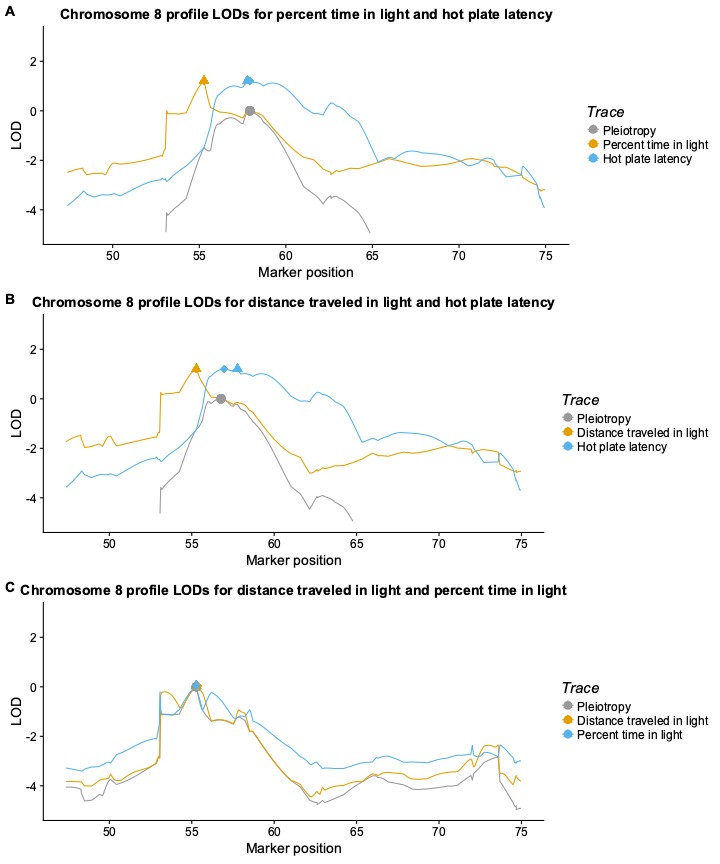
\includegraphics[width=0.5\linewidth]{all3.png}
\caption{Bootstrap p-values: 0.109, 0.108, 0.871}

\end{figure}

\end{block}

%------------------------------------------------


%----------------------------------------------------------------------------------------
%	CONCLUSION
%----------------------------------------------------------------------------------------
\setbeamercolor{block title}{fg=black,bg=orange!70} % Change the block title color


\begin{block}{Conclusions}

\begin{itemize}
\item \textit{Hydin} doesn't affect the light-dark box traits
\item A second QTL affects both light-dark box traits
\end{itemize}

\end{block}
\setbeamercolor*{block title}{fg=taorange,bg=ta2gray}


%----------------------------------------------------------------------------------------
%	REFERENCES
%----------------------------------------------------------------------------------------

\begin{block}{References}
        
%\nocite{*} % Insert publications even if they are not cited in the poster
\tiny{\bibliographystyle{apa-good}
%\tiny{\bibliographystyle{natbib}
\bibliography{sample}}

\end{block}

%----------------------------------------------------------------------------------------
%	ACKNOWLEDGEMENTS
%----------------------------------------------------------------------------------------

\begin{block}{Acknowledgments}

\begin{itemize}
  \item UW-Madison Center For High Throughput Computing 
  \item National Institutes of Health grant R01GM070683 (to K.W.B.).
\end{itemize}

\end{block}

%----------------------------------------------------------------------------------------
%	CONTACT INFORMATION
%----------------------------------------------------------------------------------------

\setbeamercolor{block title}{fg=black,bg=orange!70} % Change the block title color

\begin{block}{Contact Information}

\begin{itemize}
\item Fred Boehm
\item R package on Github: \href{https://github.com/fboehm/qtl2pleio}{https://github.com/fboehm/qtl2pleio}
\item Analysis R code on Github: \href{https://github.com/fboehm/qtl2pleio-manuscript}{https://github.com/fboehm/qtl2pleio-manuscript}
\item Website: \href{https://fboehm.us}{https://fboehm.us}
\item Email: \href{mailto:frederick.boehm@gmail.com}{frederick.boehm@gmail.com}
\end{itemize}

\end{block}

%----------------------------------------------------------------------------------------

\end{column} % End of the second column

\begin{column}{.015\textwidth}\end{column} % Empty spacer column

\end{columns} % End of all the columns in the poster

\end{frame} % End of the enclosing frame

\end{document}
